% TU Delft beamer template
% Author: Erwin Walraven (initial version was created by Maarten Abbink)
% Delft Universiy of Technology

\documentclass{beamer}
\usepackage[english]{babel}
\usepackage{calc}
\usepackage[absolute,overlay]{textpos}
\usepackage{graphicx}
\usepackage{subfig}
\usepackage{amsmath}
\usepackage{amsfonts}
\usepackage{amsthm}
\usepackage{braket}
\usepackage{epstopdf}

\usepackage{comment}
\usepackage{MnSymbol,wasysym}

\setbeamertemplate{navigation symbols}{} % remove navigation symbols
\mode<presentation>{\usetheme{tud}}

% BIB SETTINGS
\usepackage[backend=bibtex,firstinits=true,maxnames=30,maxcitenames=20,url=false,style=authoryear]{biblatex}
\bibliography{bibfile}
\setlength\bibitemsep{0.3cm} % space between entries in the reference list
\renewcommand{\bibfont}{\normalfont\scriptsize}
\setbeamerfont{footnote}{size=\tiny}
\renewcommand{\cite}[1]{\footnote<.->[frame]{\fullcite{#1}}}


\title[]{Quantum Trajectories: Fact or Fiction?}
\institute[]{Delft University of Technology, The Netherlands}
\author{Bas Dirkse \and Jaap Wesdorp}
%\date{}

\begin{document}
{
\setbeamertemplate{footline}{\usebeamertemplate*{minimal footline}}
\frame{\titlepage}
}

{\setbeamertemplate{footline}{\usebeamertemplate*{minimal footline}}

}

\begin{frame}{Outline}
\begin{itemize}
	\item Introduction to quantum noise
	\item Microscopic trajectories
	\item Density matrix entropy
	\item Discussion
\end{itemize}
\end{frame}

\section{Introduction to noise}
\begin{frame}{Open quantum systems}
	\begin{itemize}
		\item 	How to describe a non-isolated system?
		\item 	\emph{"A Description of open quantum systems in terms of a statistical average over single realizations"}
		\item We search for physical interpretations of microscopic behaviour based on ensemble behaviour (like exponential decay)
	\end{itemize}

\end{frame}

\begin{frame}{Quantum Monte Carlo Wavefunction}
		Each small time step we evolve $\bra{\psi}$ according to the following rules
		\begin{enumerate}
			\item j
		\end{enumerate}
\end{frame}


\section{Microscopic Trajectories}
\begin{frame}{Microscopic Trajectories: Excited state relaxation}
	Two level system which decays to ground state.
	Jump operator taken as (lowering)ladder operator applied to initial state.
	\begin{figure}[h]
		\centering
		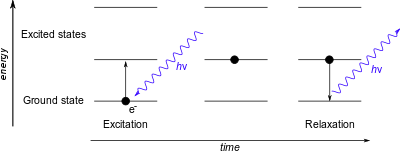
\includegraphics[width=0.6\textwidth]{figs/relaxation.png}
		\label{fig:digraph}
	\end{figure}
\end{frame}


\begin{frame}{Microscopic Trajectories: Excited state relaxation}
	
	\begin{figure}[!htb]
		\centering
		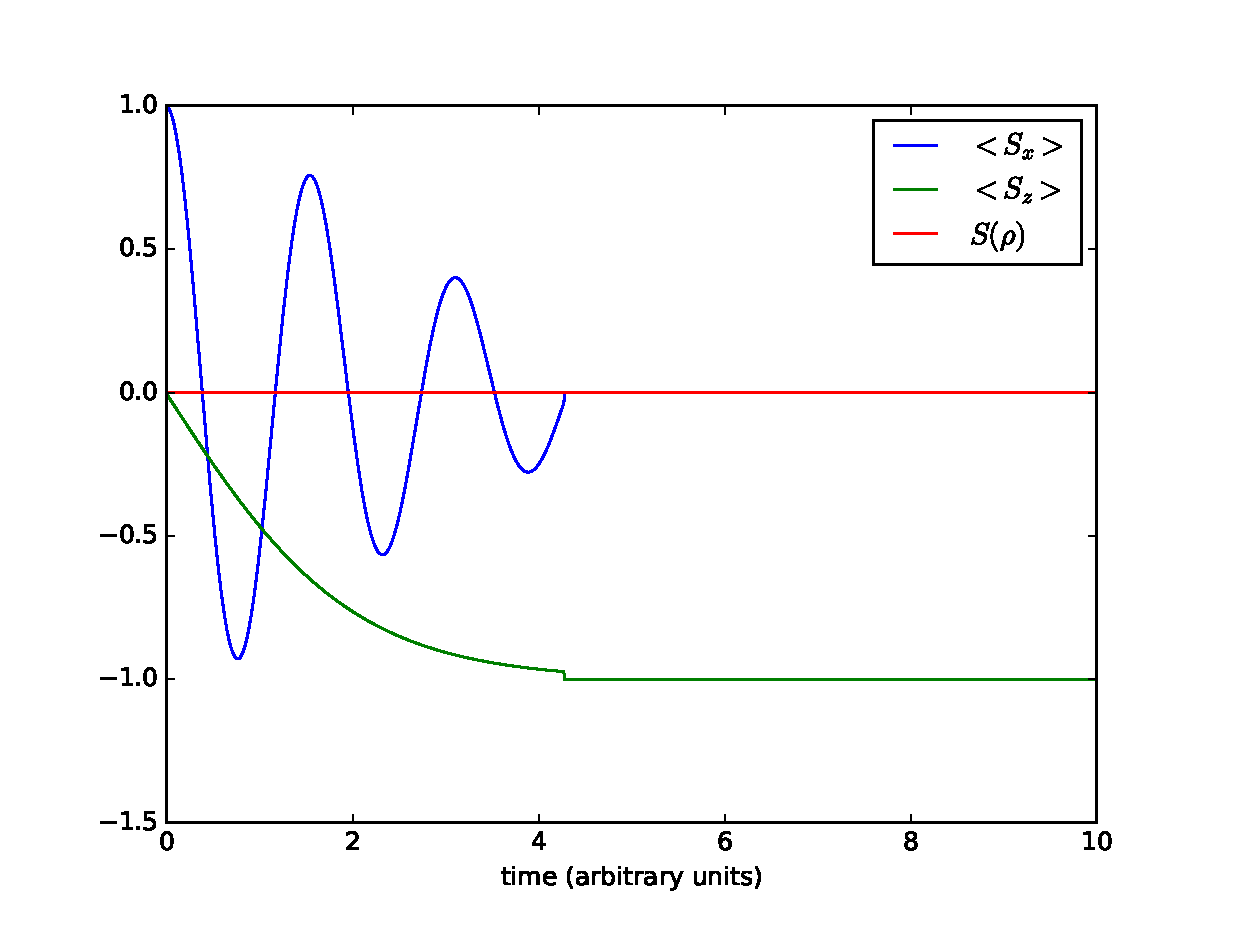
\includegraphics[width=0.7\textwidth]{figs/relaxation_1.eps}
	\end{figure}
		\begin{equation*}
		F_1 = \sigma_- =
		\begin{pmatrix}
		0 & 1 \\
		0 & 0 
		\end{pmatrix}
		\end{equation*}
\end{frame}


\begin{frame}{Microscopic Trajectories: Random phase kick}
	\begin{figure}[h]
		\centering
		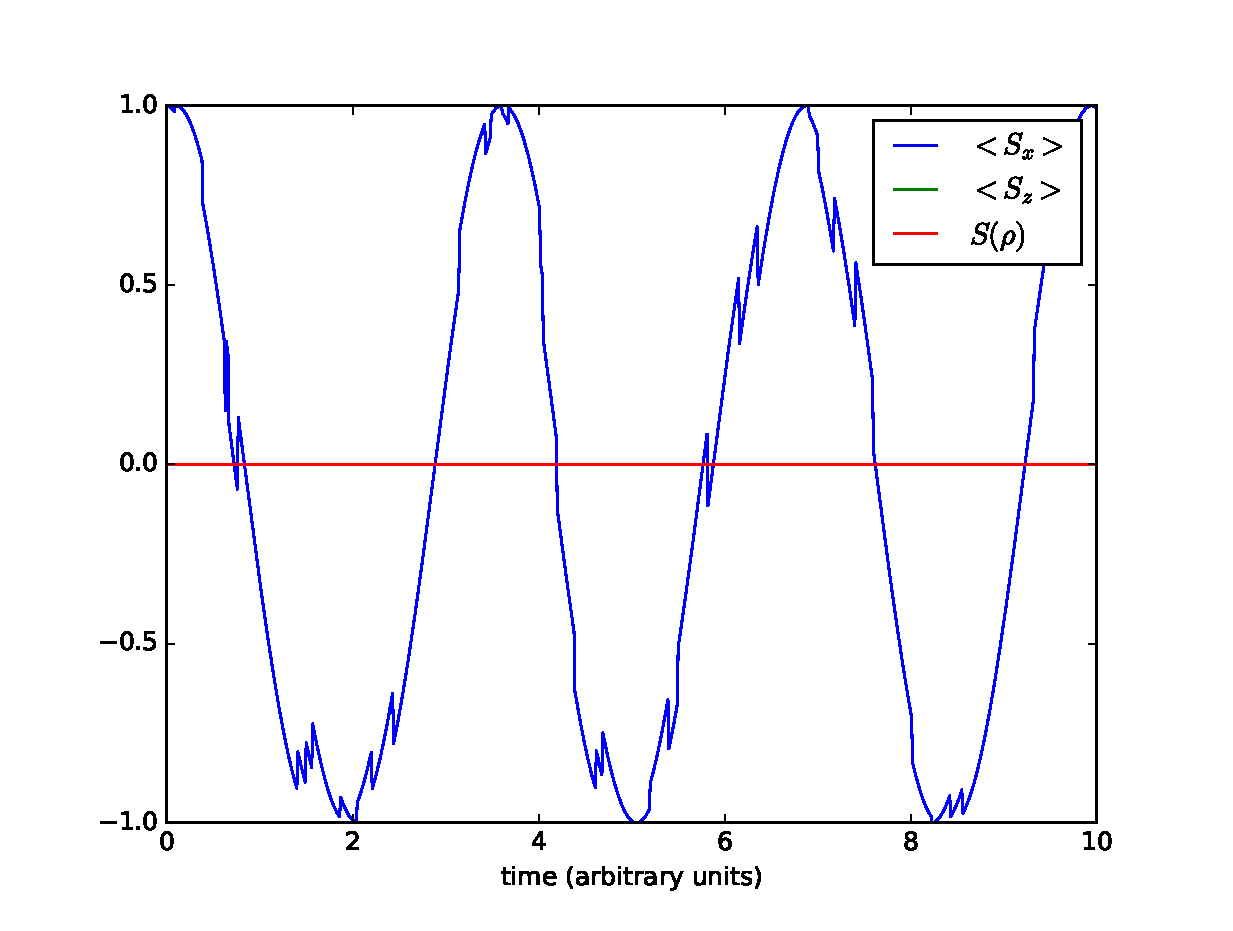
\includegraphics[width=0.7\textwidth]{figs/phase_jump_1.eps}
	\end{figure}
	\begin{equation*}
	F_1 =
	\begin{pmatrix}
	1 & 0 \\
	0 & e^{i\theta} 
	\end{pmatrix},\hspace{20pt}
	F_2 = 
	\begin{pmatrix}
	1 & 0 \\
	0 & e^{-i\theta} 
	\end{pmatrix}
	\end{equation*}
\end{frame}

\begin{frame}{Microscopic Trajectories: Phase flip}
	\begin{figure}[h]
		\centering
		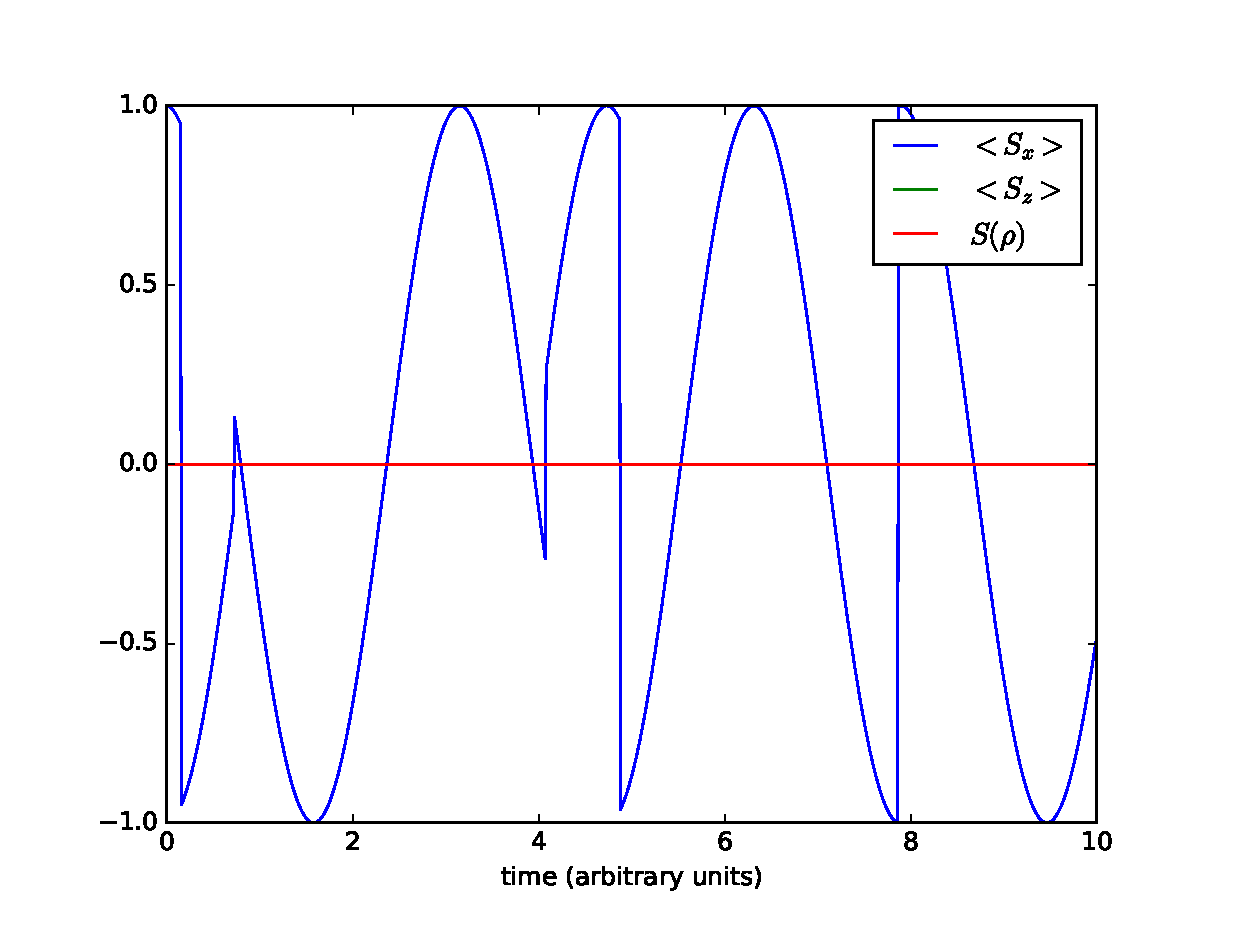
\includegraphics[width=0.7\textwidth]{figs/phase_flip_1.eps}
	\end{figure}
	\begin{equation*}
	F_1 = S_z =
	\begin{pmatrix}
	1 & 0 \\
	0 & -1 
	\end{pmatrix}
	\end{equation*}
\end{frame}
\begin{frame}{(De)coherence : Von neumann entropy}
	Measure of "known" information
	\begin{equation}
	S = -Tr(\rho \text{ln}\rho)
	\end{equation}
\end{frame}

\begin{frame}{Entropy :  phase flip average}
		\begin{figure}[h]
			\centering
			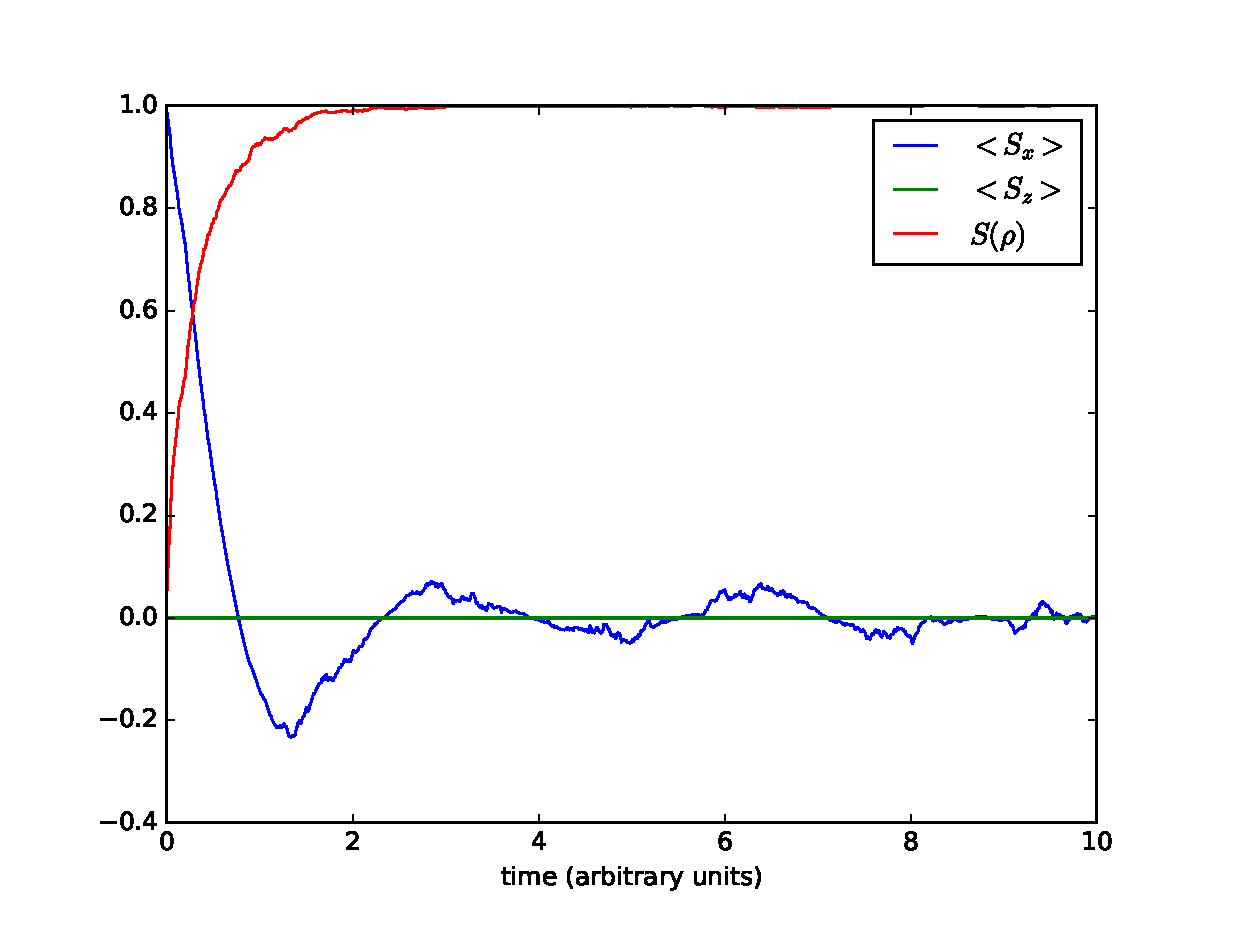
\includegraphics[width=0.7\textwidth]{figs/phase_flip_1000.eps}
		\end{figure}
\end{frame}
\begin{frame}{Entropy :  phase jump average}
	\begin{figure}[h]
		\centering
		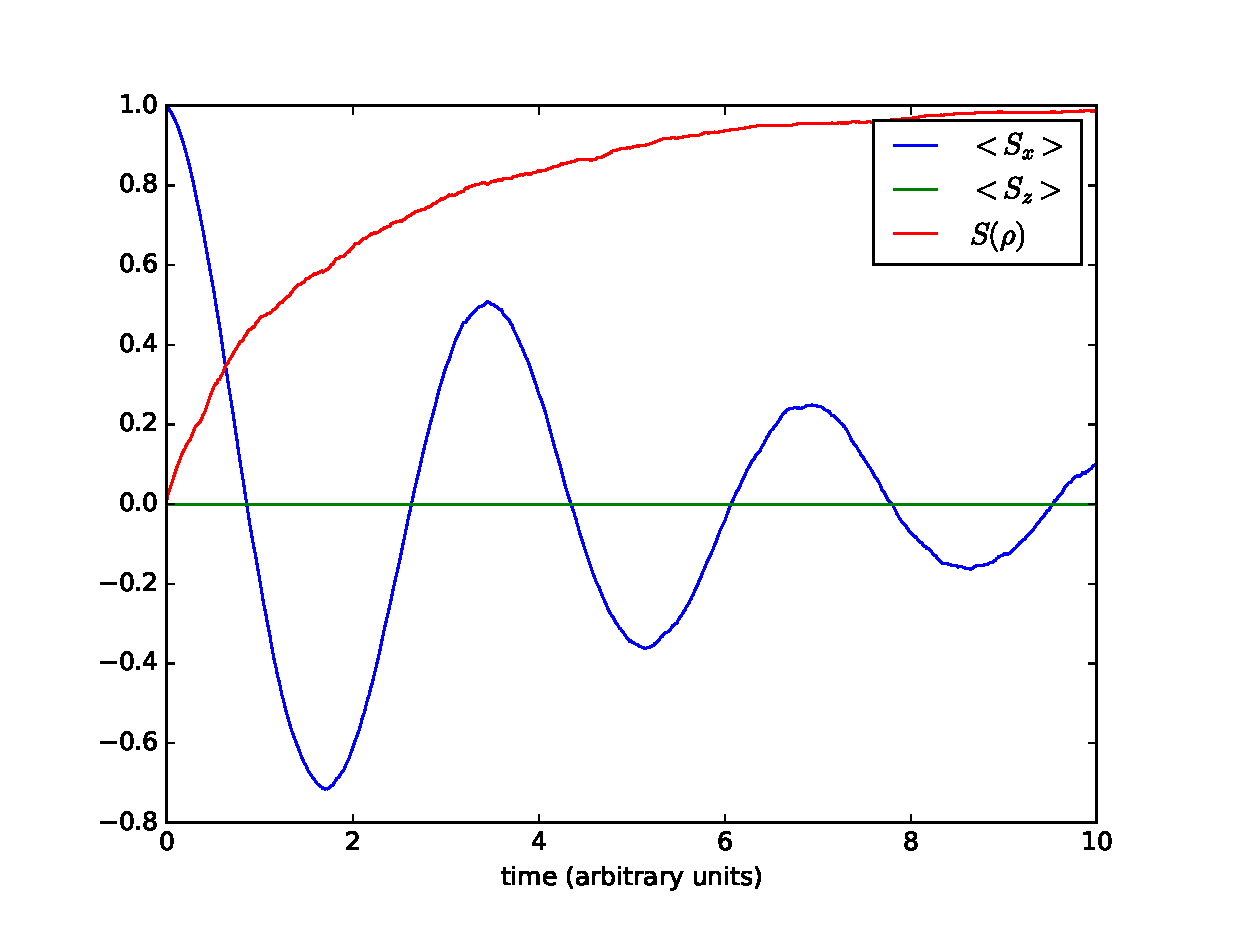
\includegraphics[width=0.7\textwidth]{figs/phase_jump_1000.eps}
	\end{figure}
\end{frame}
\begin{frame}{Entropy :  Bit Flip average}
	\begin{figure}[h]
		\centering
		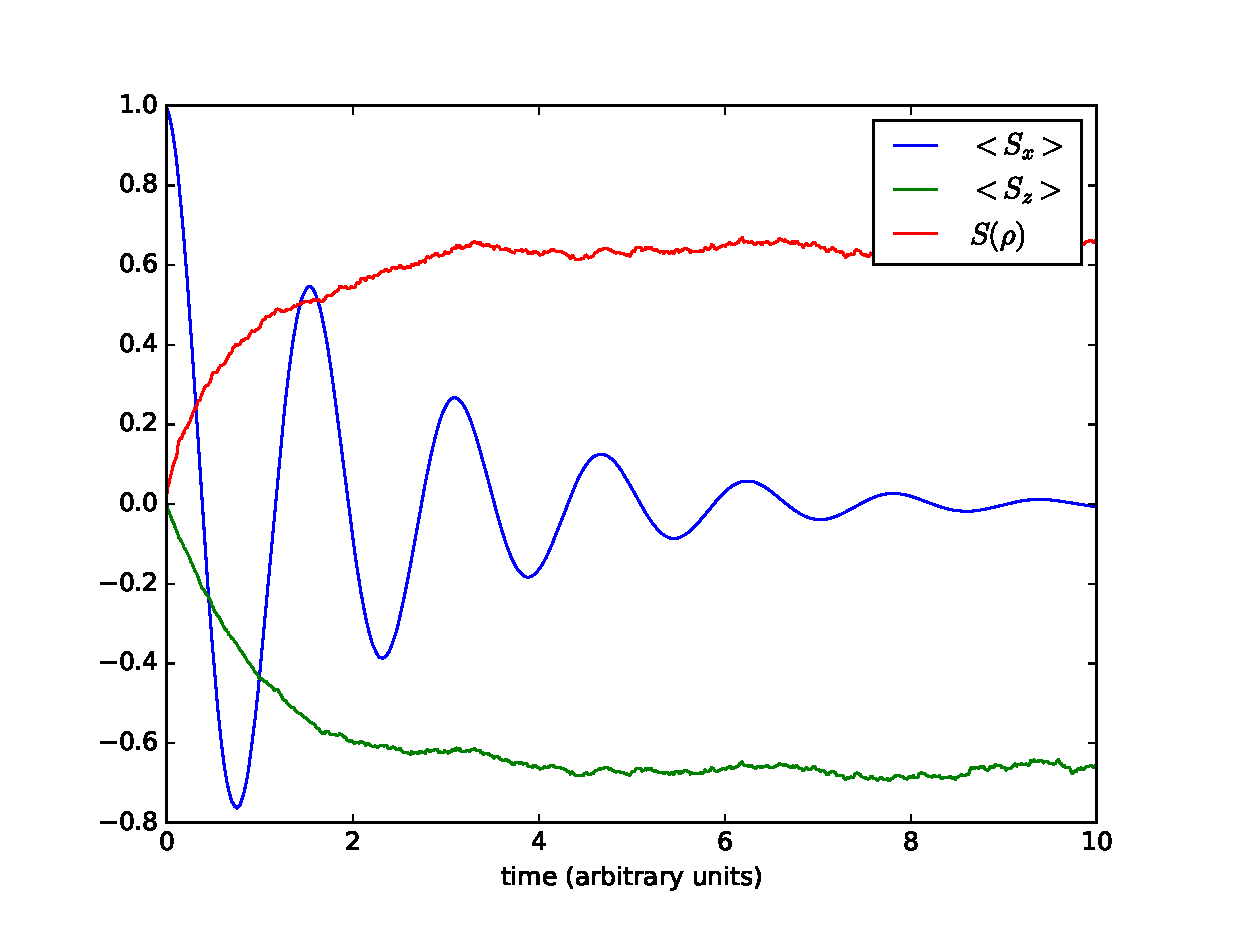
\includegraphics[width=0.7\textwidth]{figs/unequal_bitflip_1000.eps}
	\end{figure}
\end{frame}
\begin{frame}
	\begin{figure}[h]
		\centering
		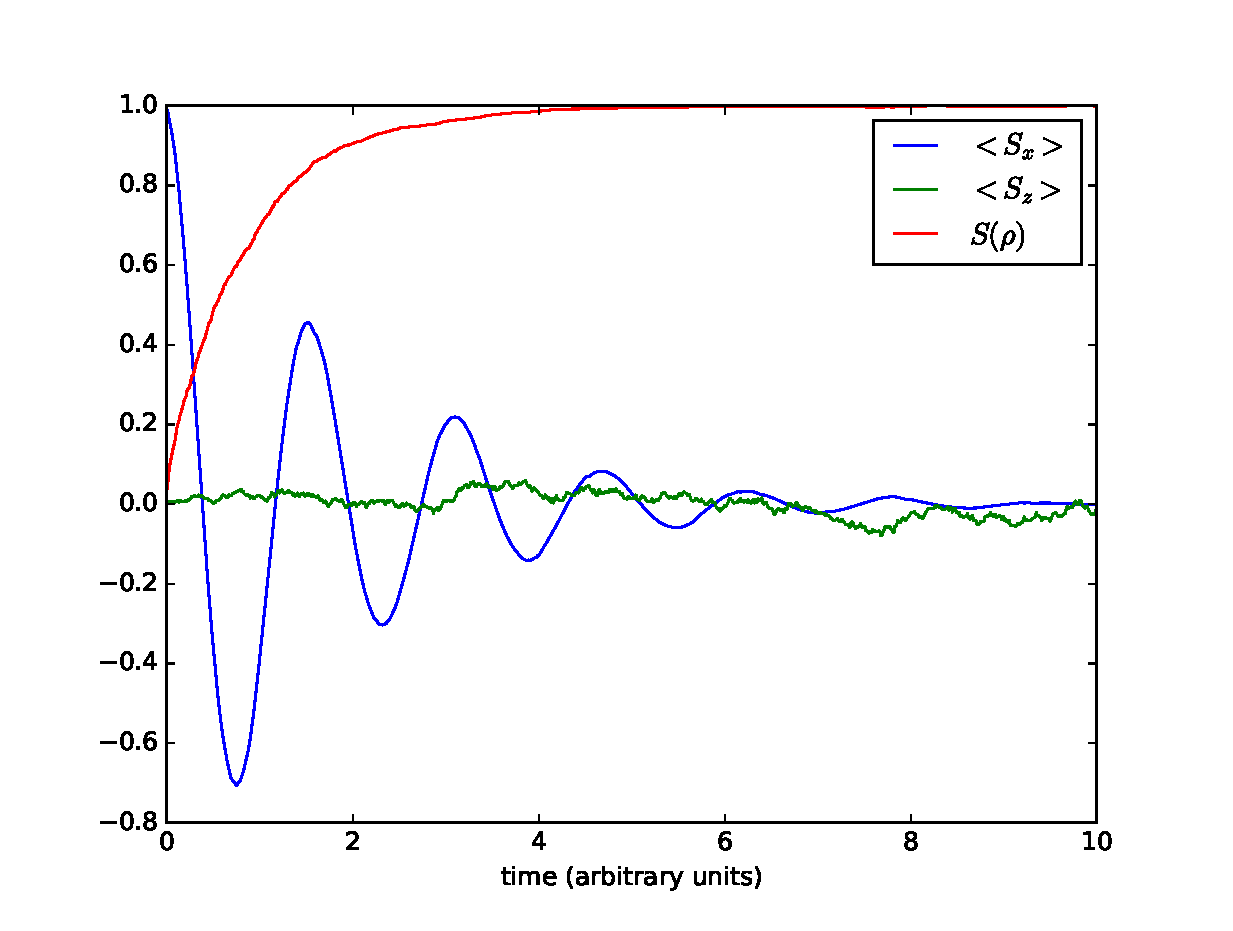
\includegraphics[width=0.7\textwidth]{figs/equal_bitflip_1000.eps}
	\end{figure}
\end{frame}
\begin{frame}{Freedom of interpretation}
	\begin{enumerate}
		\item Density matrix can be written in many ways
		\item bla?
	\end{enumerate}
\end{frame}

\end{document}
